\section{Fee Regimes}
\label{sec:fees}

\begin{figure*}[t]
\centering
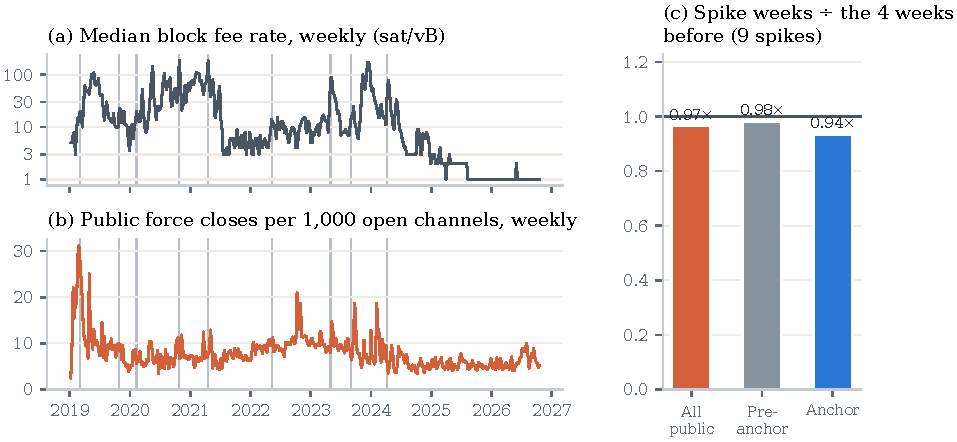
\includegraphics[width=0.9\textwidth]{figures/fig5_fee_spikes.pdf}
\caption{Fee spikes and force closes. (a) Weekly median block fee rate (log scale); vertical lines mark the spike
weeks. (b) Weekly public force closes per 1,000 open channels, mass-close events excluded. (c) Force closes in the
spike week and the week after, divided by those in the four weeks before, pooled over the \NSpikes{} spikes.}
\label{fig:spikes}
\end{figure*}

\begin{table}[t]
\centering
\caption{Fee spikes against placebos. Top: organic public force closes in a window after the spike week, divided by
the four weeks before, pooled over the spikes, against random ordinary weeks of the same years. Bottom: elasticity of
the weekly organic force-close rate to the median block fee rate, within years, by the timing of the fee rate, against
placebos that move the fee series in time.}
\label{tab:spikes}
\footnotesize
\setlength{\tabcolsep}{3.5pt}
\begin{tabular}{lrrrr}
\toprule
Weeks after spike & Spikes & Ordinary & 90\% range & Pctl. \\
\midrule
All public, 0 to +1 & \PlEvAllNow & \PlEvAllNowMed & \PlEvAllNowLo--\PlEvAllNowHi & $\PlEvAllNowPct$ \\
Pre-anchor, 0 to +1 & \PlEvLegacyNow & \PlEvLegacyNowMed & \PlEvLegacyNowLo--\PlEvLegacyNowHi & $\PlEvLegacyNowPct$ \\
Anchor, 0 to +1 & \PlEvAnchorNow & \PlEvAnchorNowMed & \PlEvAnchorNowLo--\PlEvAnchorNowHi & $\PlEvAnchorNowPct$ \\
All public, +2 to +3\textsuperscript{a} & \PlEvAllLater & \PlEvAllLaterMed & \PlEvAllLaterLo--\PlEvAllLaterHi &
$\PlEvAllLaterPct$ \\
\midrule
Fee timing & $b$ & Null 95\% (C) & Pctl.\ (C) & Pctl.\ (B) \\
\midrule
1 week later (lead) & $\PlLeadOneB$ & $\PlLeadOneCircLo$ to $\PlLeadOneCircHi$ & $\PlLeadOneCircPct$ & $\PlLeadOneBlockPct$ \\
Same week & $\PlSameWeekB$ & $\PlSameWeekCircLo$ to $\PlSameWeekCircHi$ & $\PlSameWeekCircPct$ & $\PlSameWeekBlockPct$ \\
1 week earlier & $\PlLagOneB$ & $\PlLagOneCircLo$ to $\PlLagOneCircHi$ & $\PlLagOneCircPct$ & $\PlLagOneBlockPct$ \\
2 weeks earlier & $\PlLagTwoB$ & $\PlLagTwoCircLo$ to $\PlLagTwoCircHi$ & $\PlLagTwoCircPct$ & $\PlLagTwoBlockPct$ \\
3 weeks earlier & $\PlLagThreeB$ & $\PlLagThreeCircLo$ to $\PlLagThreeCircHi$ & $\PlLagThreeCircPct$ & $\PlLagThreeBlockPct$ \\
4 weeks earlier & $\PlLagFourB$ & $\PlLagFourCircLo$ to $\PlLagFourCircHi$ & $\PlLagFourCircPct$ & $\PlLagFourBlockPct$ \\
Largest, 1--4 earlier & $\PlMaxLagB$ & $\PlMaxLagCircLo$ to $\PlMaxLagCircHi$ & $\PlMaxLagCircPct$ & $\PlMaxLagBlockPct$ \\
\bottomrule
\end{tabular}
\par\smallskip\parbox{\linewidth}{\scriptsize Ordinary: median ratio over \PlWeekDraws{} draws of one ordinary week
per spike from the same year; 90\% range of those draws. Pctl.: percentile of the real value among the draws. (C):
circular shift of the fee series, all \PlShifts{} shifts; (B): \PlBlockWeeks-week blocks shuffled within each year,
\PlBlockDraws{} draws. \textsuperscript{a}Window chosen after seeing the lag profile.}
\end{table}

\subsection{Fee spikes do not bring a wave of force closes}

\paragraph{No wave}
Fee spikes did not bring a wave of force closes. Pooled over the \NSpikes{} spikes, organic public force closes in
the spike week and the week after were \PlEvAllNow{} times their level in the four weeks before
(Table~\ref{tab:spikes}). After random ordinary weeks of the same years the ratio is typically \PlEvAllNowMed, so the
spikes sit at percentile \PlEvAllNowPct{} of those draws, below a typical week rather than above it. A wave
\PlDetectableWavePct\% above the typical ratio would have been detected. Pre-anchor channels, whose fee is fixed at
signing and which an \texttt{update\_fee} disagreement would close in a spike, show the same (\PlEvLegacyNow), as do
anchor channels (\PlEvAnchorNow). Within years, the elasticity of the weekly force-close rate to the median fee rate
of the same week is $\PlSameWeekB$, at percentile \PlSameWeekCircPct{} of a placebo that moves the fee series in
time.

\paragraph{The spikes themselves}
The spikes went both ways. \NSpikesUp{} of the \NSpikes{} came with more force closes, the most in May~2023
(\SpikeMayTwentyThreePct\% more, mostly in anchor channels), when the median fee rate went to
\SpikeMayTwentyThreeFee~sat/vB from \SpikeMayTwentyThreeFeeBefore. Next came March~2019, with \SpikeMarNineteenPct\%
more, all in pre-anchor channels and in a month when our channel list may still have been filling in. The other
\NSpikesDown{} came with fewer force closes, as many as \SpikeAprTwentyFourPct\% fewer in April~2024
(Fig.~\ref{fig:spikes}).

\paragraph{No later rise either}
Closes broadcast during a spike at too low a fee would confirm only in the weeks after it, and the chain shows
confirmation, not broadcast. Those weeks show no rise beyond placebo noise. With the fee rate of one to
four weeks earlier, the elasticity is at most $\PlMaxLagB$; tested over the four lags together, $p=\PlFwPCirc$
against the circular shift and $p=\PlFwPBlock$ against the block shuffle. In the event windows, weeks +2 to +3 reach
\PlEvAllLater{} times the weeks before, at percentile \PlEvAllLaterPct{} of ordinary weeks.

\paragraph{Unlisted closes move the other way}
Unlisted force closes fell when fees rose (elasticity $\ElastUnlisted$). Mass closes cannot be removed from them,
because their nodes are unknown, so we do not interpret this.

\subsection{Fixed commitment fees overpaid in calm markets}

\begin{figure}[t]
\centering
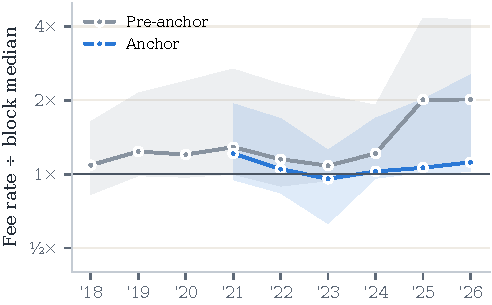
\includegraphics[width=\columnwidth]{figures/fig6_fee_guessing.pdf}
\caption{A commitment's fee rate divided by the median fee rate of the block it confirmed in, by year: median and
interquartile range, pre-anchor and anchor commitments.}
\label{fig:guessing}
\end{figure}

\paragraph{Pre-anchor commitments paid twice the market when fees were low}
Pre-anchor commitments paid a median \LegacyMedRatioEarlyMin--\LegacyMedRatioEarlyMax{} times the median fee rate of
their own block from 2018 to 2024, and \LegacyMedRatioTwentySix{} times in 2025--26 (Fig.~\ref{fig:guessing}). In
2026, \LegacyOverTwoPctTwentySix\% paid more than double, against \LegacyOverTwoPctTwentyOne\% in 2021. Over the
period, pre-anchor commitments paid \LegacyOverBtcAll~BTC more than the tenth percentile of their blocks. A commitment
that paid too little waits for a cheaper block instead, so this measure shows overpayment; underpayment shows up as
delay.

\paragraph{Anchor commitments paid about the market}
Anchor commitments paid a median \AnchorMedRatioMin--\AnchorMedRatioMax{} times their block's median. In 2023,
\AnchorBelowPTenPctTwentyThree\% confirmed below their block's tenth percentile, that is, with a child's help.

\subsection{Lightning's closing bill is small}

{\setlength{\tabcolsep}{2.5pt}\begin{table}[t]
\centering
\caption{Lightning's closing bill: fees paid by channel closes and the transactions they require, public or not, against all Bitcoin transaction fees and block space.}
\label{tab:fee_share}
\footnotesize
\begin{tabular}{lrrrrr}
\toprule
Year & Coop.\ BTC & Force BTC & Total BTC & \% of fees & \% of block space \\
\midrule
2018\textsuperscript{b} & -- & 1.39 & -- & -- & -- \\
2019 & 1.74 & 5.44 & 7.18 & 0.04 & 0.04 \\
2020 & 2.12 & 5.14 & 7.25 & 0.03 & 0.03 \\
2021 & 2.19 & 4.91 & 7.10 & 0.03 & 0.05 \\
2022 & 0.82 & 3.29 & 4.11 & 0.08 & 0.12 \\
2023 & 2.40 & 14.43 & 16.83 & 0.07 & 0.10 \\
2024 & 1.88 & 9.55 & 11.43 & 0.08 & 0.08 \\
2025 & 0.28 & 2.09 & 2.37 & 0.14 & 0.10 \\
2026\textsuperscript{a} & 0.23 & 1.29 & 1.52 & 0.18 & 0.11 \\
\bottomrule
\end{tabular}
\par\smallskip\parbox{\linewidth}{\scriptsize \textsuperscript{a}January--October. Force: commitments, required spends (split per input) and third-party anchor sweeps; cooperative closes of channels outside our public list cannot be seen and are not included, nor are channel opens. \textsuperscript{b}From 12 January; cooperative closes of 2018 are mostly outside our list, so only force closes are shown.}
\end{table}
}

\paragraph{A fraction of a percent of Bitcoin's fees}
All closes and the spends they require, public or not, with third-party anchor sweeps, paid \BillBtcTwentyThree~BTC
in 2023, the most in any year, and \BillBtcTwentySix~BTC in the first ten months of 2026 (Table~\ref{tab:fee_share}). In
every year that was \BillFeePctMin--\BillFeePctMax\% of all transaction fees and at most \BillVbPctMax\% of block
space. The share of fees rose in the low-fee years because everything else became cheaper faster.
